\section{Validation and Simulation}
\label{sec:component_diagrams-validation}

\subsection{Static Validation of diagram}
The static model validation checks that the model is well formed. The validation can be invoked at any time by clicking the V icon in the toolbar menu (see Figure \ref{fig:TheComponentDiagramEditor}). The validation is also invoked as a preliminary check when the generator is invoked. The validation rules fall into two categories; omissions that result in a meaningless model (reported as errors) and contraventions of the conventions of the components modelling notation that nevertheless can be translated to a meaningful Event-B model (reported as warnings). If the validation results in errors the generation does not proceed. If the validation raises warnings but no errors the generation proceeds. Note that model validation does not attempt to verify consistency properties of the model that will be checked by the Event-B static checker. The following validation rules are applied:

\textbf{Errors}

\begin{itemize}
\item The label of any labelled element (e.g. operations adopt a label from the events that they elaborate) shall not be null.
\item The name of any named element (e.g. Component, Connector) shall not be null.
\item The connector reference of a DataPacket (used in port sends and port wakes) shall not be null.
\item The value reference of a DataPacket shall not be null.
\item The delay value of a DelayedDataPacket (used in port sends) shall not be null.
\item The delay value of a WakeEvent shall not be null.
\item The wakeKind value of a WakeEvent shall not be null.
\item The type value of a Connector shall not be null.
\item The initial value of a Connector shall not be null.
\end{itemize}


\textbf{Warnings}

\begin{itemize}
\item An operation shall only send data to a connector that is an outgoing connector for the component that contains the operation
\item An operation shall only call methods that are contained in the component that contains the calling operation or in one of its sub-components.
\item A PortWake operation shall have at least one port wakeup.
\item A PortWake operation shall only receive port wakeups from a connector that is an incoming connector for the component that contains the PortWake operation.
\end{itemize}


\subsection{Model checking using ProB}
The ProB model checker can be used to verify the generated Event-B model. ProB is initiated by right clicking on a machine and then selecting Start Animation / Model Checking. The layout of the Rodin interface (perspective) should change to one similar to that shown in Figure \ref{fig:ProBModelCheckerInterface}.
 
\begin{figure}[!htbp]
  \centering
  \ifplastex
  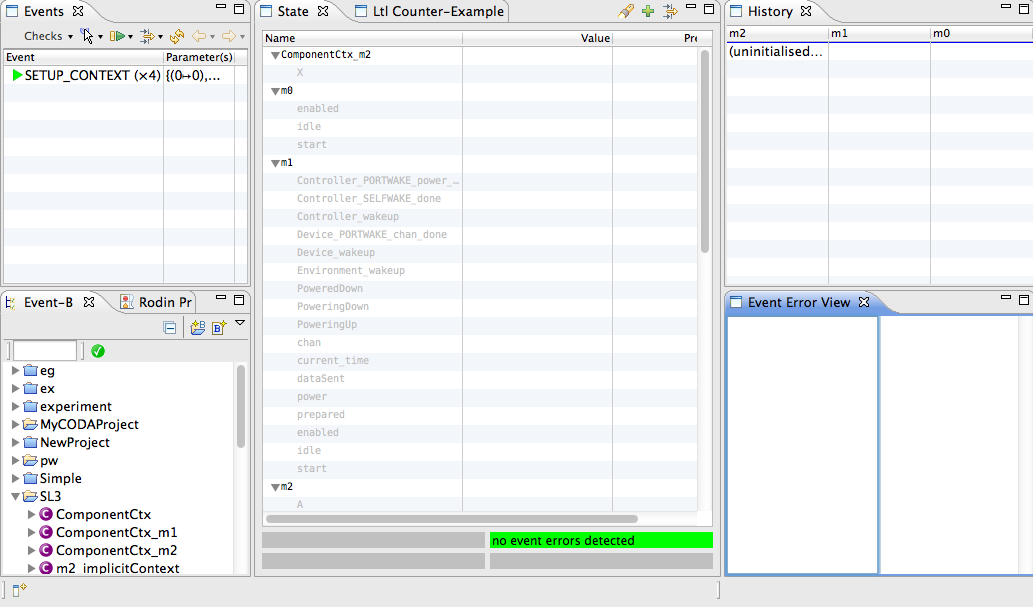
\includegraphics[width=1024]{figures/image8.png}
  \else
  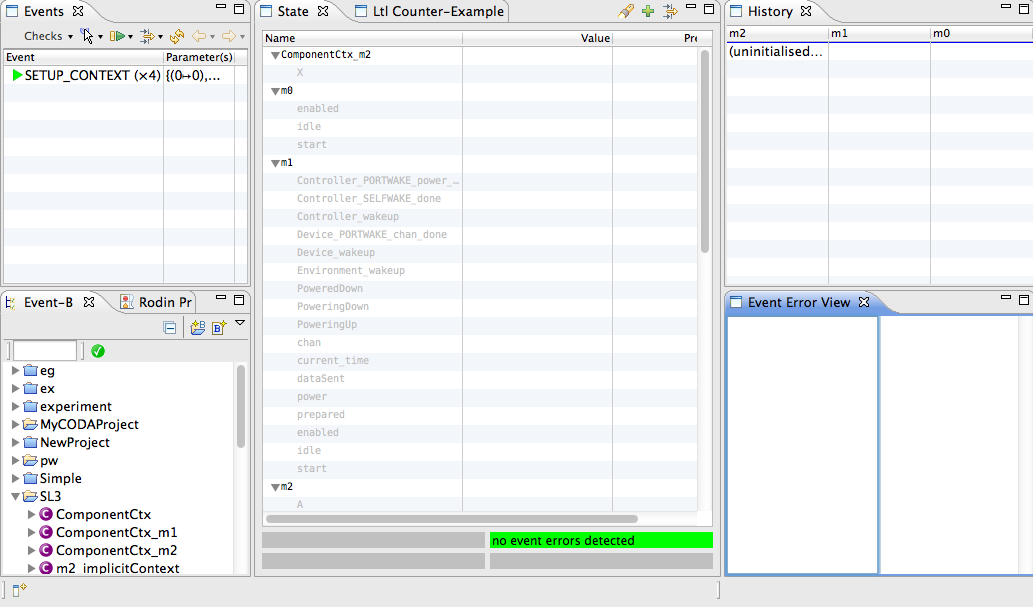
\includegraphics[width=1\textwidth]{figures/image8.png}
  \fi
  \caption{ProB Model Checker Interface}
  \label{fig:ProBModelCheckerInterface}
\end{figure}


The model can be animated by manually selecting enabled events from the view in the top left and observing the changes to the state in the centre view. However, it is recommended that the Oracle simulator is used for animation because it provides a higher-level interface oriented on the component model.
Model checking is invoked using the drop down menu from the checks toolbar item in the top-left Events view. The model checking options will then be displayed in a new window. Typical settings of these options are shown in Figure \ref{fig:ProBModelCheckerOptions}.

 
 \begin{figure}[!htbp]
  \centering
  \ifplastex
  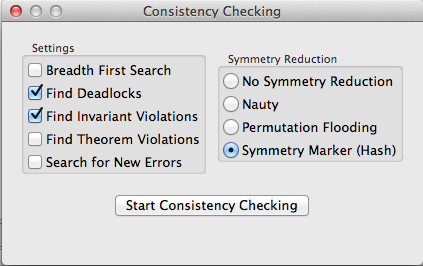
\includegraphics[width=512]{figures/image9.png}
  \else
  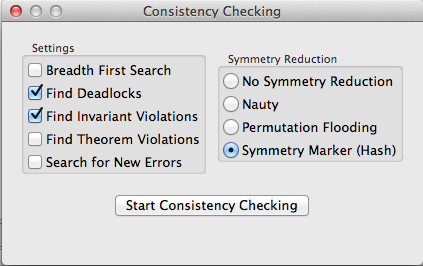
\includegraphics[width=0.5\textwidth]{figures/image9.png}
  \fi
  \caption{ProB Model Checker Options}
  \label{fig:ProBModelCheckerOptions}
\end{figure}


The generated model contains an infinite state space (due to the indefinite incrementing of time) and therefore the model checker will not complete its search of the state space. The model checker should be stopped manually after a short period and the coverage statistics can be examined to see the extent of coverage of the model. Since model checking does not complete it does not ensure that the model is consistent or deadlock free. However, the model checker often finds problems quickly and is therefore useful when trying to find problems in a model.
More details about running the ProB model checker are given here\footnote{\url{http://www.stups.uni-duesseldorf.de/ProB/index.php5/User_Manual}}.


\subsection{State-machine Animation}


State-machines may be animated by clicking the running man icon in the toolbar menu (see Figure \ref{fig:TheComponentDiagramEditor}). The currently active state (if any) is shown with a bold outline (Figure \ref{fig:StatemachineAnimationInterface}). Any enabled transitions (i.e. transitions that are linked to at least one event that is enabled) are shown in green and the event may be selected for execution by clicking on the transition and selecting from the pop-up list. The state-machine animation is a view to the Pro-B model checker and during animation, all of the Pro-B interface is also available. Usually the state-machine will only represent part of the model and it will be necessary to fire some events from the ProB Events view when no transitions are enabled. State-machine animation provides a clearer view of the behaviour of the state-machine part of the model so that its interaction with other variables and events of the model can be validated. State-machine animation is not essential but may be a useful optional validation step.
 
 \begin{figure}[!htbp]
  \centering
  \ifplastex
  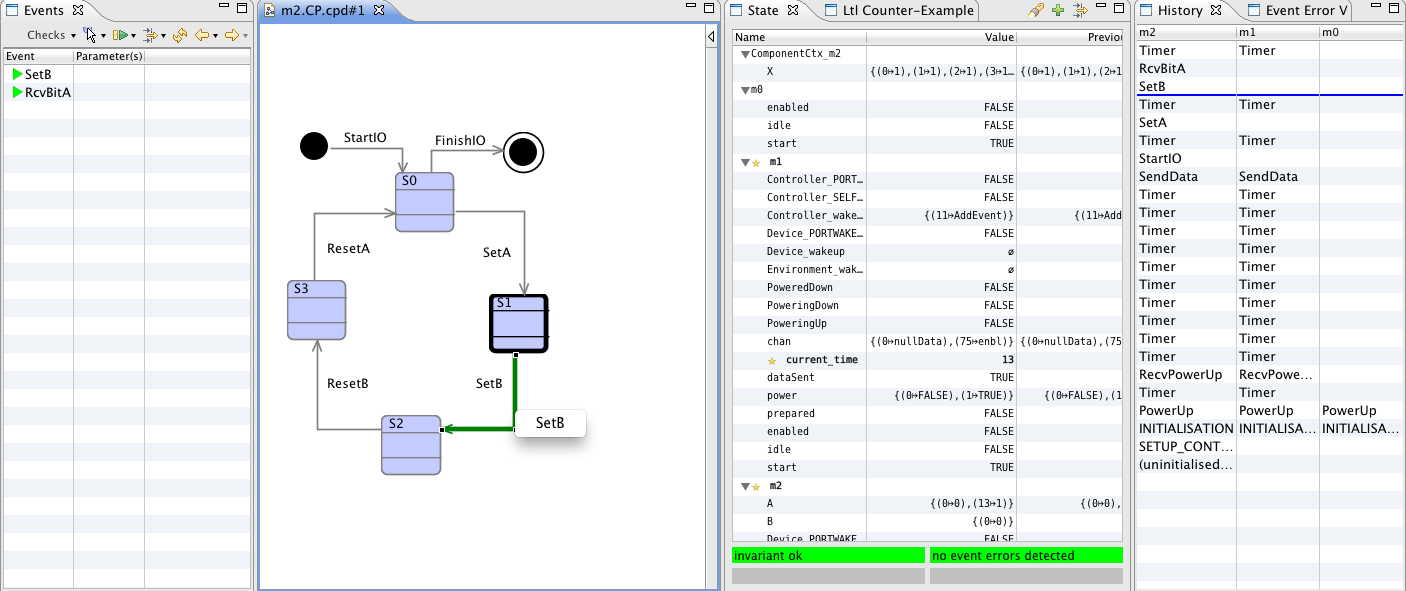
\includegraphics[width=1024]{figures/image10.png}
  \else
  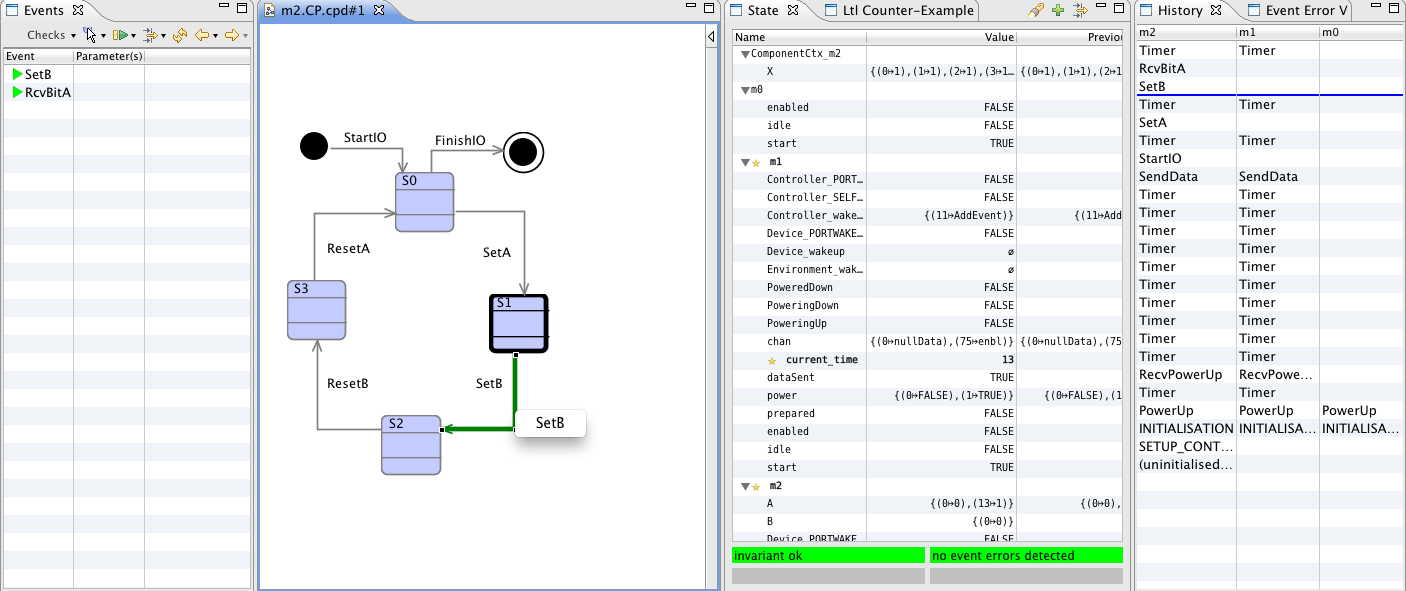
\includegraphics[width=1.0\textwidth]{figures/image10.png}
  \fi
  \caption{State-machine Animation Interface}
  \label{fig:StatemachineAnimationInterface}
\end{figure}

The animation can be terminated by clicking the stood man icon in the toolbar menu (see Figure \ref{fig:TheComponentDiagramEditor}).


\subsection{Simulation of Component model}
The CODA simulator is based on ProB but provides an interface that is aware of the CODA components model. The interface consists of an additional view that is presented as part of the ProB perspective (the lower view in Figure \ref{fig:CODASimulatorUserInterface}). The simulator is started by right clicking on a machine and selecting \textbf{Simulation-Start}. 
 
 \begin{figure}[!htbp]
  \centering
  \ifplastex
  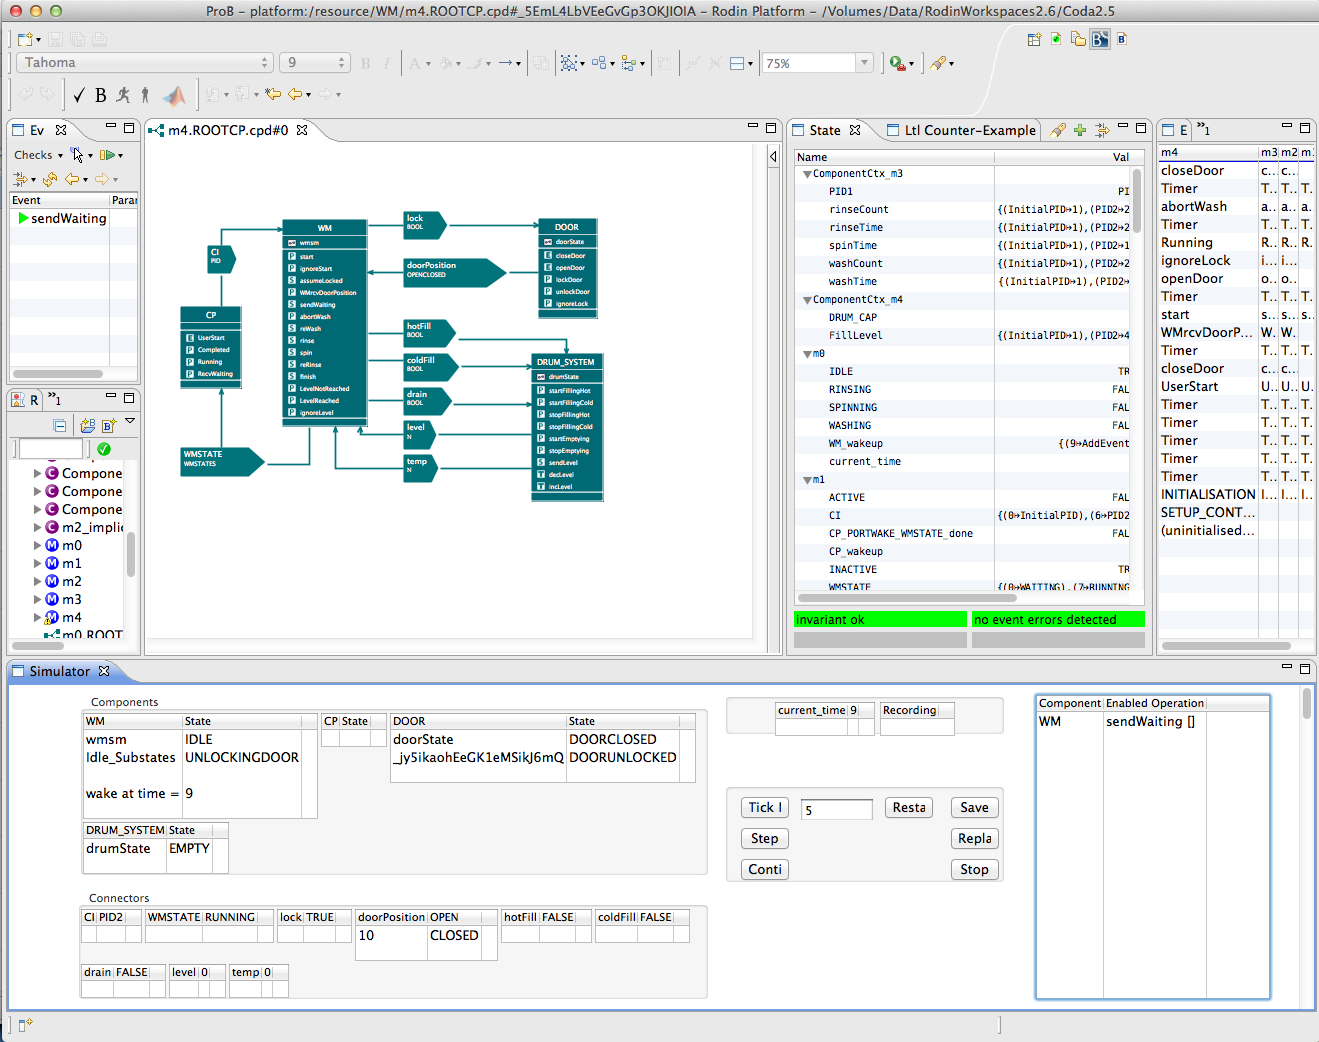
\includegraphics[width=1024]{figures/image11.png}
  \else
  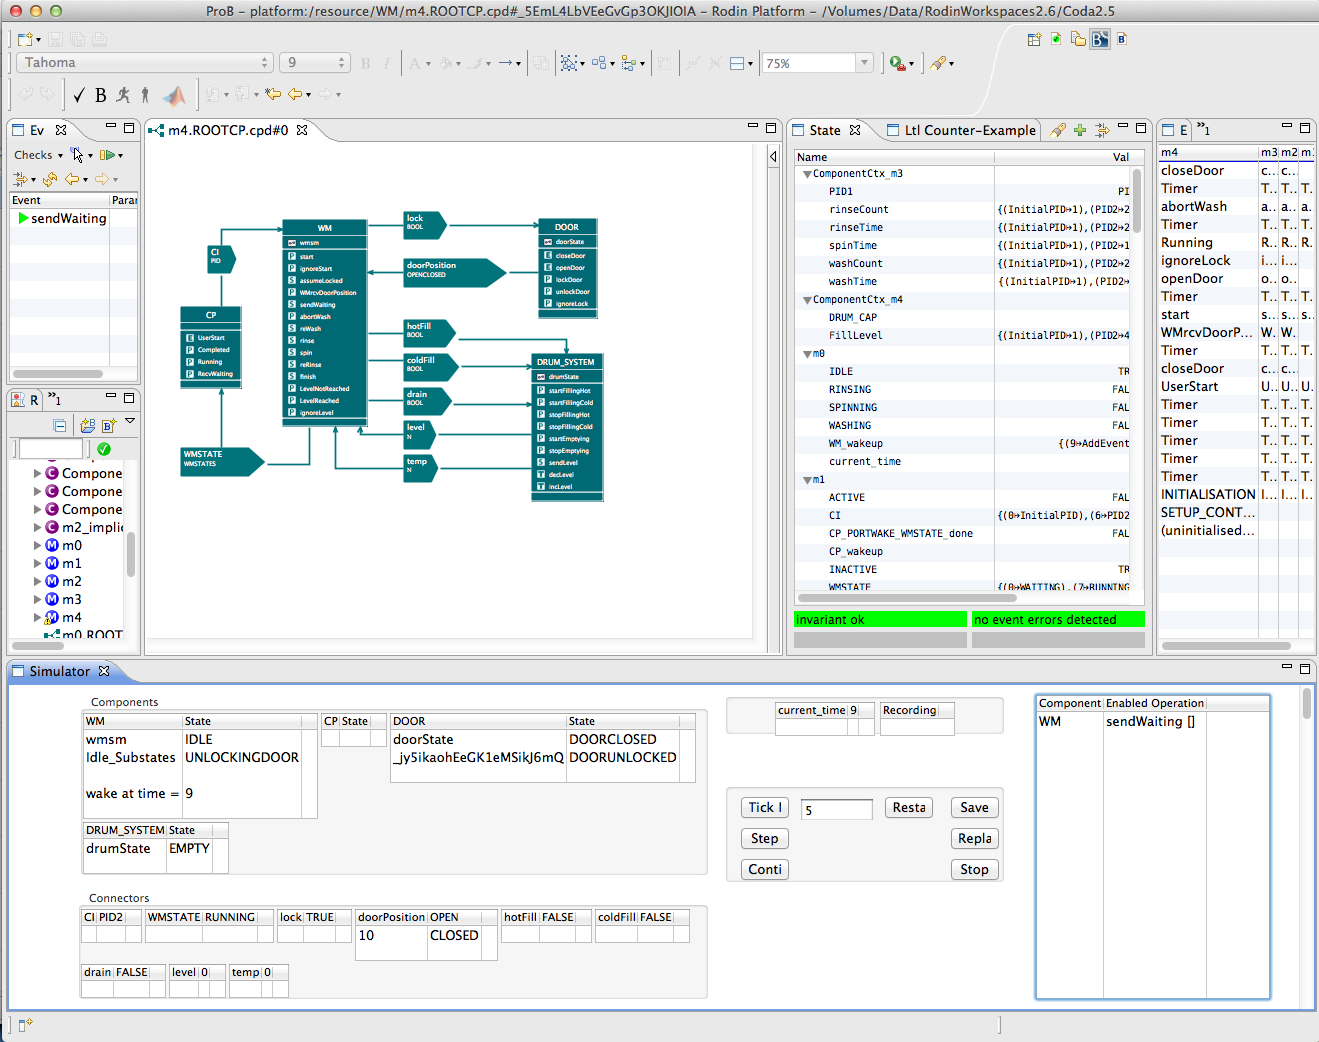
\includegraphics[width=1\textwidth]{figures/image11.png}
  \fi
  \caption{CODA Simulator User Interface}
  \label{fig:CODASimulatorUserInterface}
\end{figure}


5.4.1	Modes

During simulation there are two modes. Recording, where a new gold run is being recorded or playback where a previous gold run is being replayed for comparison. During recording the user controls which operations execute whereas during playback the system controls which operations execute.  The simulation modes and effect of control buttons is shown in Figure \ref{fig:ModelOfCODASimulatorOperation}.

 \begin{figure}[!htbp]
  \centering
  \ifplastex
  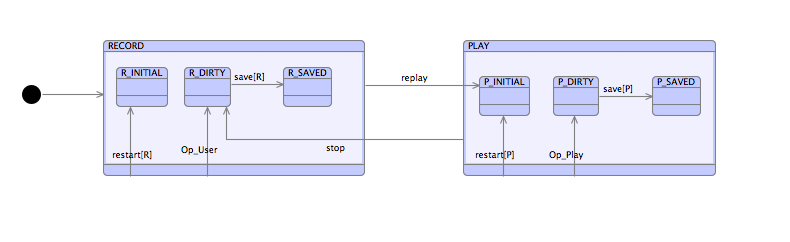
\includegraphics[width=1024]{figures/image12.png}
  \else
  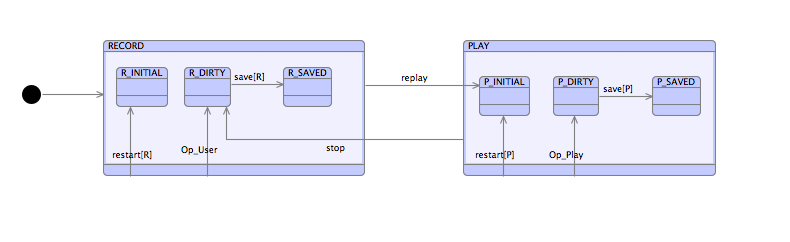
\includegraphics[width=1\textwidth]{figures/image12.png}
  \fi
  \caption{Model of CODA Simulator Operation}
  \label{fig:ModelOfCODASimulatorOperation}
\end{figure} 

5.4.2	Recording Mode

During recording mode, operations can be invoked manually from the enabled operations table or via one of the three left hand buttons on the control panel. These buttons have the following functions. Tick N selects operations non-deterministically from those that are enabled until the clock has advanced by the number of clock ticks configured in the adjacent panel. Step selects one operation non-deterministically from those that are enabled. Continue, selects operations non-deterministically from those that are enabled until a choice between two operations of the same component is required. To ensure the latter button terminates a limit (20) of the number of operations is applied. 
At any point the gold run can be saved by pressing the Save button or discarded by pressing the Restart or Replay buttons. The Restart button remains in record mode and the Replay button switches to playback mode.

5.4.3	Playback Mode

During playback mode, a previous gold run is selected and its operations are replayed. Operations may not be selected from the enabled operations table. The three buttons in the control panel have slightly different behaviour. Tick N selects operations from the sequence defined in the gold run until the clock has advanced by the number of clock ticks configured in the adjacent panel. Step selects the next operation from the gold run. Continue, selects operations from the gold run until it is exhausted or the limit (20) of the number of operations is reached.
At any point the playback run can be saved by pressing the Save button or discarded by pressing the Restart button. The Restart button remains in playback mode. At any time (whether saved or not) the playback can be left and continued in record mode by pressing the Stop button. This enables a previous gold recording to be extended or a different branch to be taken at any point.

5.4.4	Summary of Control Buttons
\begin{itemize}
\item Save - [recording | playback] Saves the current trace model and continues in the same mode. (The trace model is a gold run when in recording mode and a normal run in playback mode.
\item Stop - [playback] Leaves playback and continues in recording mode. (The trace from playback is continued so that it can be extended to make a new gold run). When in recording mode, does nothing.
\item Restart - [recording | playback] Discards the current trace and re-starts animation in the same mode as before. (In playback mode, the same gold run is replayed).
\item Replay - [recording] Leaves recording mode and enters playback mode. The current trace is discarded and reset. A gold run for playback is chosen and loaded via a user dialog.
\end{itemize}

5.4.5	Saved Trace runs

The gold and playback runs are saved into a folder, called Oracle in the project that is being simulated. The file names for the runs are auto generated using the following scheme.

Gold runs:

\texttt{<Machine name>.test.<timestamp>.gold_oracle}

Playback runs:

\texttt{<Machine name>.test.<timestamp>.oracle}


%%% Local Variables:
%%% mode: latex
%%% TeX-master: "component_diagrams-user_manual"
%%% End:
